
\section*{Aufgabe 1}

Gegeben seien die folgenden beiden Normen im \( \mathbb{R}^2 \):

\begin{itemize}
    \item Betragssummennorm/Manhattan-Norm (1-Norm):
    \[
    \left\| \begin{pmatrix} x_1 \\ x_2 \end{pmatrix} \right\|_1 = |x_1| + |x_2|
    \]

    \item Maximumnorm/Unendlich-Norm (\(\infty\)-Norm):
    \[
    \left\| \begin{pmatrix} x_1 \\ x_2 \end{pmatrix} \right\|_\infty = \max\{|x_1|, |x_2|\}
    \]
\end{itemize}

Die zugehörigen Metriken erhält man durch \( d(\mathbf{x}, \mathbf{y}) = \|\mathbf{x} - \mathbf{y}\| \).

\subsection*{Einheitskreise}

Der Einheitskreis ist die Menge \( K = \{\mathbf{x} \mid d(\mathbf{x}, \mathbf{0}) = 1\} \) aller Punkte, die den Abstand 1 vom Koordinatenursprung haben. Die Einheitskreise für jede Metrik sehen wie folgt aus:

\begin{center}
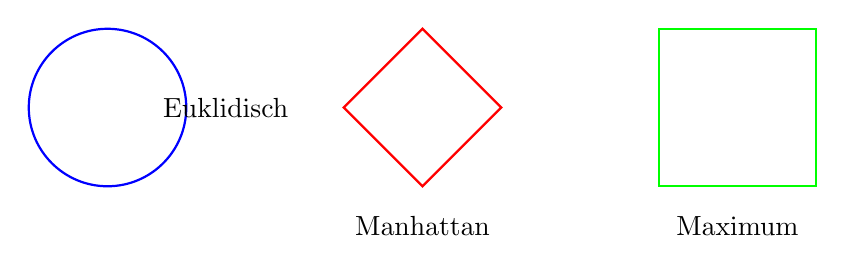
\begin{tikzpicture}
% Euklidischer Einheitskreis
\draw[thick,blue] (0,0) circle(1);
\node at (1.5,0) {Euklidisch};

% Manhattan Einheitskreis
\begin{scope}[xshift=4cm]
\draw[thick,red] (1,0) -- (0,1) -- (-1,0) -- (0,-1) -- cycle;
\node at (0,-1.5) {Manhattan};
\end{scope}

% Maximum Einheitskreis
\begin{scope}[xshift=8cm]
\draw[thick,green] (-1,-1) rectangle (1,1);
\node at (0,-1.5) {Maximum};
\end{scope}
\end{tikzpicture}
\end{center}

Die dargestellten Einheitskreise zeigen die Unterschiede in den Metriken:
\begin{itemize}
    \item Der euklidische Einheitskreis ist ein normaler Kreis mit Radius 1.
    \item Der Manhattan Einheitskreis bildet eine Raute (Diamantform).
    \item Der Maximum Einheitskreis bildet ein Quadrat.
\end{itemize}
